\footnotesize
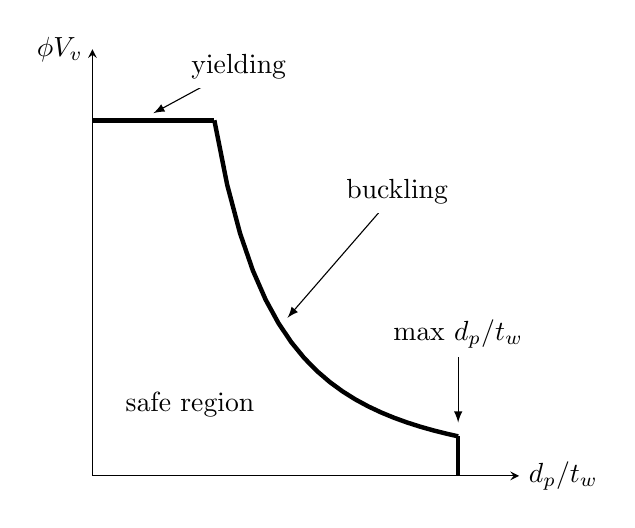
\begin{tikzpicture}[>=latex]
\begin{axis}[
width=7cm,
height=7cm,
xtick=\empty,
ytick=\empty,
axis x line=center,
axis y line=center,
xlabel={$d_p/t_w$},
ylabel={$\phi{}V_v$},
xlabel style={right},
ylabel style={left},
xmin=0,xmax=3.5,ymin=0,ymax=1.2]
\addplot[ultra thick,domain=1:3,samples=20]{1/x/x};
\draw[ultra thick](axis cs:0,1)--(axis cs:1,1);
\draw[ultra thick](axis cs:3,0)--(axis cs:3,1/9);
\draw[<-](axis cs:.5,1.02)--(axis cs:1.2,1.15)node[fill=white]{yielding};
\draw[<-](axis cs:1.6,4/9)--(axis cs:2.5,.8)node[fill=white]{buckling};
\draw[<-](axis cs:3,.15)--(axis cs:3,.4)node[fill=white]{max $d_p/t_w$};
\node at(axis cs:.8,.2){safe region};
\end{axis}
\end{tikzpicture}